\documentclass[tikz,border=8pt]{standalone}
\usepackage{amsmath}
\usetikzlibrary{arrows.meta,calc,patterns}

\begin{document}
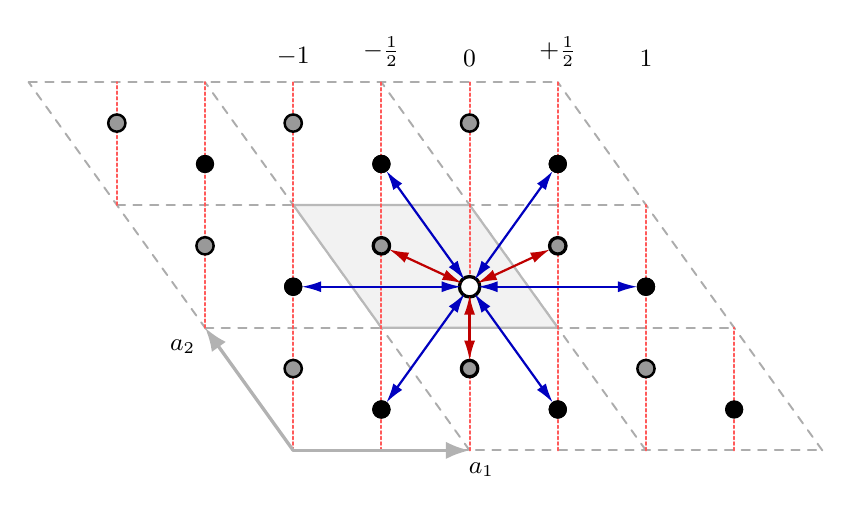
\begin{tikzpicture}[
    x=1.12cm, y=0.9cm,
    line cap=round, line join=round,
    cell/.style={draw=gray!65, dash pattern=on 3pt off 3pt, line width=0.7pt},
    cellhl/.style={draw=gray!55, line width=0.8pt, fill=gray!10},
    plane/.style={draw=red!65, dash pattern=on 1pt off 1pt, line width=0.7pt},
    siteA/.style={circle, fill=black, draw=black, inner sep=2.2pt},
    siteB/.style={circle, fill=black!40, draw=black, line width=0.9pt, inner
    sep=2.2pt},
    vac/.style={circle, fill=white, draw=black, line width=1.2pt, inner sep=2.6pt},
    vec/.style={very thick, draw=gray!60, -{Latex[length=3mm,width=2.2mm]}},
    basal/.style={thick, draw=blue!75!black,
        {Latex[length=2.5mm,width=1.4mm]}-{Latex[length=2.5mm,width=1.4mm]}},
    inter/.style={thick, draw=red!75!black,
        {Latex[length=2.5mm,width=1.4mm]}-{Latex[length=2.5mm,width=1.4mm]}},
    lbl/.style={font=\small}
]

\def\a{2}
\coordinate (a1) at (\a,0);
\coordinate (a2) at ({-0.5*\a},{0.8660254*\a});

% 3x3 primitive-cell grid around the central cell
\foreach \j in {-1, 0, 1, 2} {
    \coordinate (u\j) at
        ({\j*(-0.5*\a) - \a}, {\j*0.8660254*\a});
    \draw[cell] (u\j) --
        ({\j*(-0.5*\a) + 2*\a}, {\j*0.8660254*\a});
}

\foreach \i in {0, 1, 2, 3} {
    \coordinate (v\i) at ({\i*\a - 0.5*\a}, {-0.8660254*\a});
    \draw[cell] (v\i) -- ({\i*\a - 2*\a}, {2*0.8660254*\a});
}

% highlight the central primitive cell
\draw[cellhl] (0,0) -- (a1) -- ($(a1)+(a2)$) -- (a2) -- cycle;

% draw vertical planes through each basis atom
% shorten the first two vertical lines to fit cell grid
\coordinate (vl) at ({-1.5*\a}, {0.8660254*\a});
\draw[plane] (vl) -- ({-1.5*\a}, {2*0.8660254*\a});
\coordinate (ul) at ({-\a}, {0.});
\draw[plane] (ul) -- ({-\a}, {2*0.8660254*\a});
\foreach \i in {0, 1} {
    \coordinate (v\i) at ({\i*\a - 0.5*\a}, {-0.8660254*\a});
    \draw[plane] (v\i) -- ({\i*\a - 0.5*\a}, {2*0.8660254*\a});
    \coordinate (u\i) at ({\i*\a}, {-0.8660254*\a});
    \draw[plane] (u\i) -- ({\i*\a}, {2*0.8660254*\a});
}
\foreach \x/\lab in {{-1}/{$-1$},{-0.5}/{$-\tfrac12$},{0}/{$0$},{0.5}/{$+\tfrac12$},{1}/{$1$}} {
    \node[lbl, anchor=south] at ({(\x + 0.5)*\a}, {2.05*0.8660254*\a}) {\lab};
}
% shorten the last two vertical lines to fit cell grid
\coordinate (vr) at ({1.5*\a}, {-0.8660254*\a});
\draw[plane] (vr) -- ({1.5*\a}, {0.8660254*\a});
\coordinate (ur) at ({2*\a}, {-0.8660254*\a});
\draw[plane] (ur) -- ({2*\a}, {0.});
% direct coordinates in the local primitive-cell basis
% original: A = (-1/2, -1/2), B = (-1/6, 1/6)
% direct shift by +a2 means add (0,1) in direct coordinates.
% shifted positions: A' = (-1/2, 1/2), B' = (-1/6, 7/6)
% apply the Cartesian shift s = -(1/6)(a2 - a1) = (a/4, -sqrt(3)a/12)
% then translate everything by +a along the Cartesian x-axis.
\coordinate (A) at ({-0.5*\a + 0.5*(-0.5*\a) + 0.25*\a + \a}, {0.5*0.8660254*\a - 0.144337567*\a});
\def\rint{0.57735*\a}
\coordinate (B) at ($(A)+({\rint*cos(150)},{\rint*sin(150)})$);
% hcp basis atoms in all visible primitive cells
 \foreach \i in {-1,0,1} {
     \foreach \j in {-1,0,1} {
         \coordinate (Ai\i\j) at ($(A)+\i*(a1)+\j*(a2)$);
         \coordinate (Bi\i\j) at ($(B)+\i*(a1)+\j*(a2)$);
         \node[siteA] at (Ai\i\j) {};
         \node[siteB] at (Bi\i\j) {};
     }
 }

% restore the vacancy symbol over the A atom at the jump origin
\node[vac] at (A) {};
% \node[siteB] at (B) {};

% all jump vectors move together with the shifted atomic position A
% 6 same-plane NN sites around the vacancy in the basal plane
\foreach \ang in {0,60,120,180,240,300} {
  \coordinate (N\ang) at ($(A)+({\a*cos(\ang)}, {\a*sin(\ang)})$);
  \node[siteA, fill=black] at (N\ang) {};
  \draw[basal, shorten <=3pt, shorten >=3pt] (A) -- (N\ang);
}

% projected interplanar NN positions: only 3 directions remain after projection,
% because the +z and -z neighbors in each azimuth overlap in the 2D view.
\foreach \m in {0,1,2} {
  \pgfmathsetmacro{\ang}{30 + 120*\m}
  \coordinate (I\m) at ($(A)+({\rint*cos(\ang)}, {\rint*sin(\ang)})$);
  \node[siteB, inner sep=2pt] at (I\m) {};
  \draw[inter, shorten <=3pt, shorten >=3pt] (A) -- (I\m);
}

% draw lattice vectors a1 and a2 in their previous position
\draw[vec] ({-1*\a + -1*(-0.5*\a)}, {-1*0.8660254*\a}) -- ({-1*\a + -1*(-0.5*\a) + \a}, {-1*0.8660254*\a});
\draw[vec] ({-1*\a + -1*(-0.5*\a)}, {-1*0.8660254*\a}) -- ({-1*\a + -1*(-0.5*\a) + (-0.5*\a)}, {-1*0.8660254*\a + 0.8660254*\a});
\node[lbl, anchor=south west] at ({-1*\a + -1*(-0.5*\a) + \a - 0.12}, {
    -1*0.8660254*\a - 0.5}) {$a_1$};
\node[lbl, anchor=south east] at ({-1*\a + -1*(-0.5*\a) + (-0.5*\a)}, {-1*0.8660254*\a + 0.8660254*\a - 0.5}) {$a_2$};

\end{tikzpicture}
\end{document}
